\section{Introduction}
\label{sec:introduction}

\begin{figure*}
    \centering
    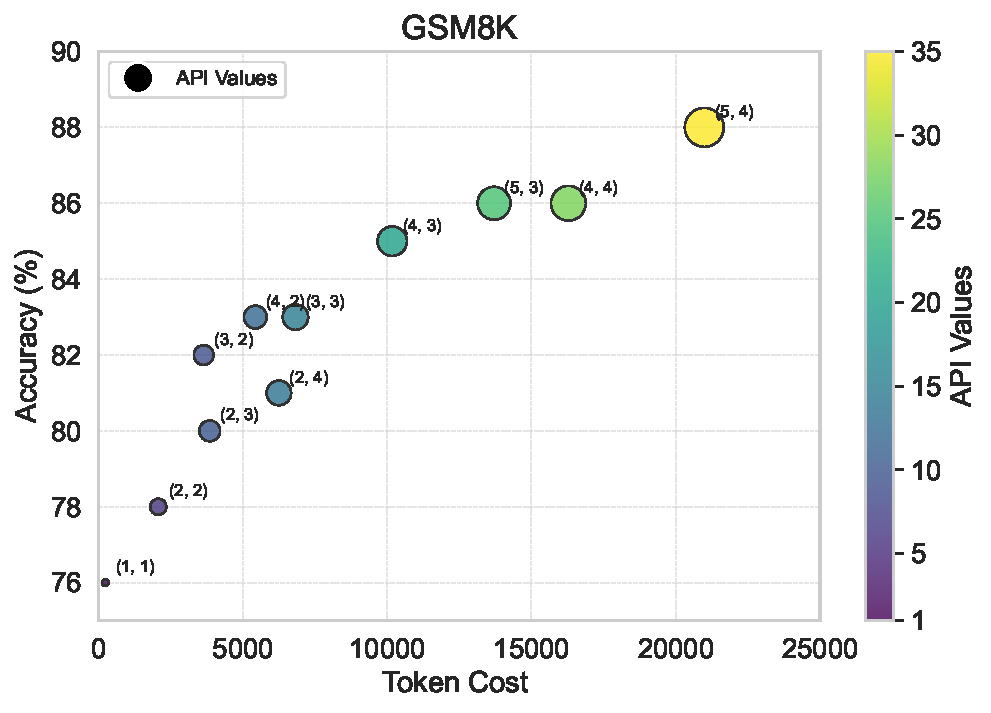
\includegraphics[width=0.48\linewidth]{figs/GSM8K_1.pdf}
    \hfill
    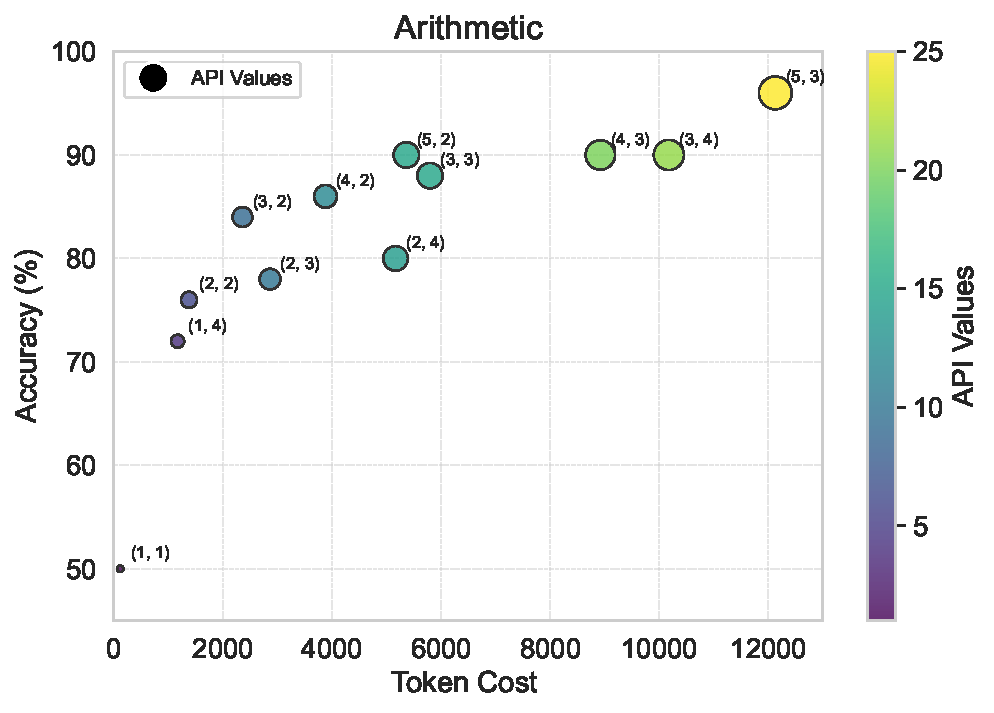
\includegraphics[width=0.48\linewidth]{figs/Arithmetic_1.pdf}
    \caption{\textbf{Comparison of Token Cost and Accuracy Under Different Combinations of Agents and Rounds.} The numbers in parentheses corresponding to each circle represent the pair of agent number and round number. The size/color of the circle represents the number of API calls, indicating that the larger the circle, the more times the OpenAI API is called.}
    \label{fig1}
\end{figure*}

Large language Models (LLMs) such as GPT \cite{openai2024gpt4,brown2020language,bubeck2023sparks,radford2018improving,radford2019language}, LLaMa \cite{touvron2023llama,touvron2023llama2}, and PaLM \cite{anil2023palm,chowdhery2023palm} have revolutionized the field of natural language processing (NLP) by demonstrating remarkable capabilities across a wide range of tasks. These models can reach or even exceed human performance in a range of NLP tasks but their performance is still limited in complex mathematical and logical reasoning tasks \cite{liu2023evaluating}. To address these limitations, researchers have proposed developed various techniques to enhance the reasoning abilities of LLMs. Chain-of-Thought \cite{kojima2023large,wei2023chainofthought,nye2021work} encourages models to generates the reasoning process step by step. Subsequent research has introduced such as Tree-of-Thoughts \cite{yao2024tree} and Verification \cite{lightman2023lets} to enhance their ability to perform complex multi-step reasoning. Unfortunately, these single-agent methods are more likely to fall into random fabrication of facts or the generation of delusions, thus leading to erroneous outcomes \cite{bubeck2023sparks,huang2023survey,ji2023survey}. 
The multi-agent debate methods mitigate these issues by allowing different agents to express their arguments to each other and these approaches have demonstrated considerable potential and effectiveness across various types of tasks and datasets \cite{chan2023chateval,du2023improving,liang2023encouraging,sun2023corex,wang2023apollo,xiong2023examining,xu2023toward}.

% \begin{figure*}
%     \centering
%     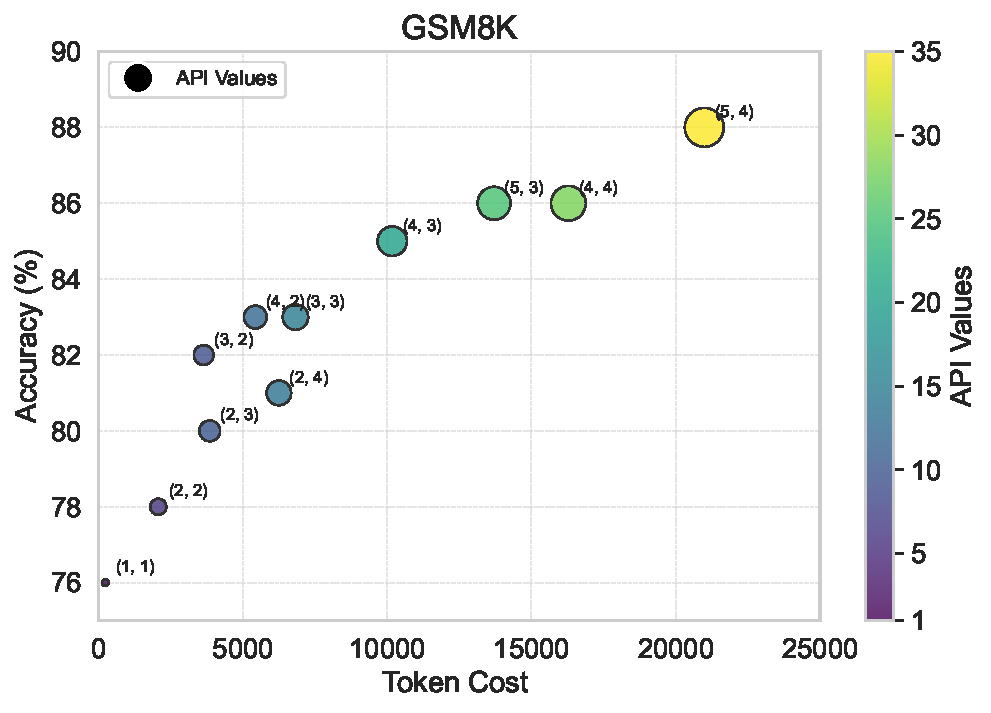
\includegraphics[width=0.48\linewidth]{figs/GSM8K_1.pdf}
%     \hfill
%     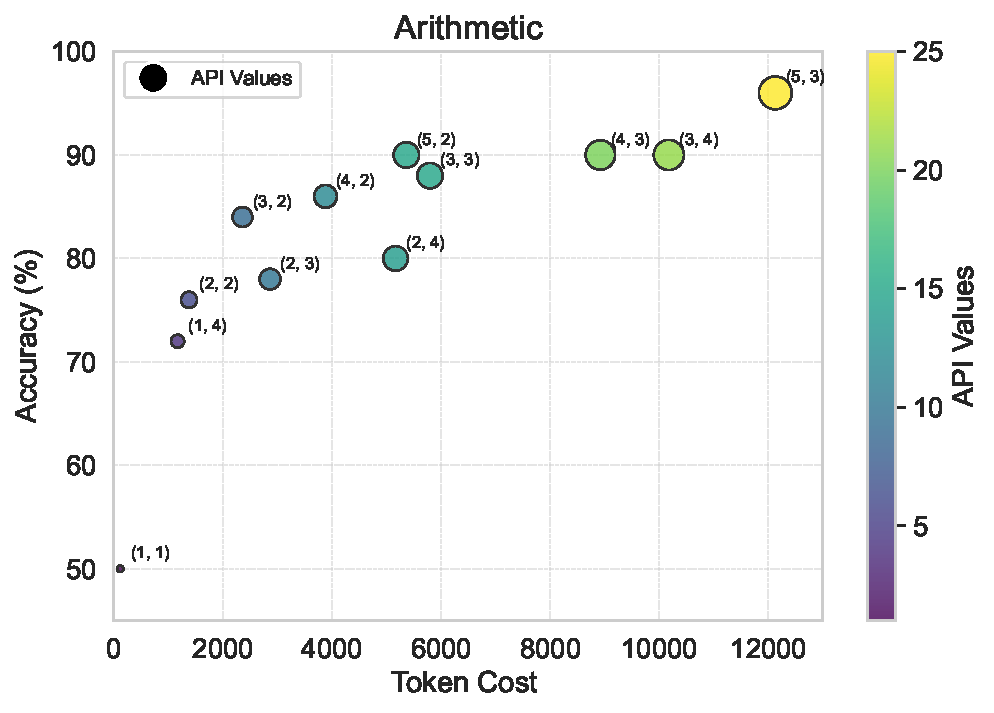
\includegraphics[width=0.48\linewidth]{figs/Arithmetic_1.pdf}
%     \caption{\textbf{Comparison of Token Cost and Accuracy Under Different Combinations of Agents and Rounds.} The numbers in parentheses corresponding to each circle represent the pair of agent number and round number. The size/color of the circle represents the number of API calls, indicating that the larger the circle, the more times the OpenAI API is called.}
%     \label{fig1}
% \end{figure*}

However, as the number of agents and rounds increases, the token cost in multi-agent debate can escalate significantly. This issue results in monetary expenditure on tokens through LLM-based API or substantial computational overhead and power consumption, thereby severely hindering the scalability and broader application of multi-agent debate, especially in scenarios with limited computational resources \cite{guo2024large}.
As illustrated in the Figure \ref{fig1}, compared with a single LLM-based agent, employing a multi-agent debate with three agents in five rounds can potentially raise the accuracy from the initial 50\% to 98\%, but introduces 101× token cost in the Arithmetic \cite{brown2020language} task. Similarly, in the GSM8K \cite{cobbe2021training} task, five rounds of multi-agent debate involving four agents can raise the accuracy from 76\% to 88\%, but it results in 90× token cost. To address the issue of the rapidly increasing number of tokens in multi-agent debates, researchers have proposed various improved techniques. For instance, the multi-agent debate in \cite{du2023improving} summarizes the output of other agents to serve as the input for the next round. \cite{sun2023corex} proposes a "forgetfulness" mode that only the output from the previous round is stored as input for the next round. 
However, only employing a "forgetfulness" mode or summary mechanism to reduce token cost is still limited due to their theoretical complexity and the issue of exacerbated token growth. Moreover, owing to their simplistic debating modes, they struggle to fully exploit the collaborative capabilities of multi-agent debates.

In human societies, when multiple individuals engage in a debate, they usually conduct group discussion to enhance the efficiency of interaction while also preserving the diversity of viewpoints \cite{krueger2014focus}. Inspired by this, in this paper, we propose a novel method GroupDebate (GD), which leverages group discussion to further reduce token cost in multi-agent debates. Specifically, Our method divides all participating agents into several debate groups, with each group conducting internal debates. Following the debates, the results are summarized and placed into a shared pool. After that, each group of agents retrieves the debate summaries of all groups from the pool, which serve as the input for the agents in the next round. Upon the conclusion of the debate, all agents reach a consensus or the final outcome is determined by majority vote. Furthermore, we conduct a theoretical analysis of the total token cost of the GroupDebate, thereby affirming the effectiveness of the method. In our experiments, we evaluate the effectiveness of GroupDebate in comparison to existing multi-agent debate methods and observe up to 34.8\%/45.2\%/46.9\%/39.3\%/30.6\% reduction in token cost in the Arithmetic/GSM8K/MMLU/MATH/GPQA dataset, as well as up to 12\%/21.9\% improvement in accuracy in the MMLU/GPQA dataset. 

Our main contributions are as follows: 

\begin{itemize}
    \item[1.] We propose an innovative multi-agent debate strategy GroupDebate based on group discussion which can improve the efficiency and performance of multi-agent debates.
    \item[2.] We conduct a theoretical analysis of token cost based on our method, demonstrating its efficiency and effectiveness.
    \item[3.] Extensive experiments across five logical reasoning and mathematical datasets show that our method can not only significantly reduce token cost but also potentially enhance accuracy, validating the efficiency and superiority of our method.
\end{itemize}